%
Given ellipse is
\begin{align}
   \vec{x}^T\myvec{9&0\\0&4}\vec{x}=36
\end{align}
%
On comparing it with standard form we have,
\begin{align}
    \vec{V}=\myvec{9&0\\0&4},\vec{u}=0,f=-36\\
    \implies\vec{u}^T\vec{V}^{-1}\vec{u}-f = 36\\
    \implies\vec{c} = -\vec{V}^{-1}\vec{u} = \myvec{0\\0}\\
\end{align}
The eigen vector decomposition of 
\begin{align}
    \vec{V} = \myvec{9&0\\0&4}
\end{align}
is given by
\begin{align}
    \vec{D} &= \myvec{9&0\\0&4} \implies \lambda_1 = 9,\lambda_2 = 4\\
    \vec{P} &= \myvec{1&0\\0&1}\implies \vec{p}_1 = \myvec{1\\0}, \vec{p}_2 = \myvec{0\\1}
\end{align}
Since
\begin{align}
   \lambda_1 > \lambda_2
\end{align}
Eccentricity of the ellipse is,
\begin{align}
   e &= \sqrt{1-\frac{\lambda_2}{\lambda_1}}
   = \frac{\sqrt{5}}{3}
\end{align} 
Semi major and minor axes of ellipse are,
\begin{align}
    a = \sqrt{\frac{\vec{u}^{\top}\vec{V}^{-1}\vec{u}-f}{\lambda_2}} = 3\\ 
    b = \sqrt{\frac{\vec{u}^{\top}\vec{V}^{-1}\vec{u}-f}{\lambda_1}} = 2
\end{align}
The co-ordinates of vertices are,
\begin{align}
   \pm\myvec{0 \\ 3} 
\end{align}
The co-ordinates of foci are given by,
\begin{align}
  \vec{F}  = \frac{ce^2\vec{n}-\vec{u}}{\lambda_1}
\end{align}
Where,
\begin{align}
    \vec{n} &= \sqrt{\lambda_1}\vec{p}_2
\end{align}
\begin{multline}
     c = \frac{e\vec{u}^{\top}\vec{n} \pm \sqrt{e^2\brak{\vec{u}^{\top}\vec{n}}^2-\lambda_2\brak{e^2-1}\brak{\norm{\vec{u}}^2 - \lambda_2 f}}}{\lambda_2e\brak{e^2-1}} 
\end{multline}
Substituting we have,
\begin{align}
    \vec{n} &= \myvec{0\\3}\\ c &= \pm\frac{27}{\sqrt{5}}\\
    \vec{F} &= \pm\myvec{0 \\ \sqrt{5}}.
\end{align}
See Fig.   \ref{sep/2/27/fig:RSUencountered}. 
\begin{figure}[t!]
  \centering
  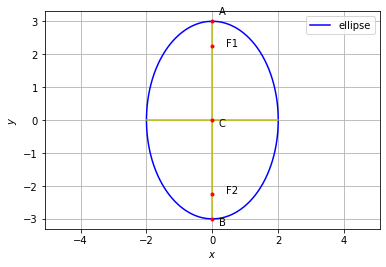
\includegraphics[ width=\columnwidth]{solutions/sep/2/27/figures/ellipse.png}
  \caption{Plot of the ellipse}   
  \label{sep/2/27/fig:RSUencountered} 
\end{figure}
